% !TEX root=./adl.tex

\section{Supervised Fine-Tuning}

\subsection{Motivation}

% -----------------------------------------------------------------------
\begin{frame}{Where Are We? Supervised Fine-Tuning}
  \llmtrainingstages{sft}

  \vspace{0.2em}
  After pretraining we hold a \emphdef{base model}: a powerful next-token predictor of web text.
  It is \emph{not} yet a helpful assistant.
  \begin{itemize}[nosep]
    \item \emphdef{Supervised fine-tuning (SFT)}: continue training on curated
      \emphdef{instruction--response} and \emphdef{dialogue} examples.
    \item Same objective as pretraining (per-token cross-entropy), new data and format.
    \item Goal: teach the model to \emphdef{follow instructions} and \emphdef{hold a conversation}.
  \end{itemize}
  \sourceref{Instruction tuning: FLAN \cite{wei2022flan}, InstructGPT \cite{ouyang2022instructgpt}}
\end{frame}

% -----------------------------------------------------------------------
\begin{frame}{Base Model vs.\ Assistant}
  A base model only \emph{continues} text. Prompt it like a chatbot and it may just
  extend the question instead of answering it.
  \begin{center}
    \begin{tikzpicture}[
      scale=0.9, every node/.style={scale=0.9},
      prompt/.style={rectangle, draw, rounded corners, fill=blue!12, align=left, font=\scriptsize, text width=4.1cm, inner sep=5pt},
      cont/.style={rectangle, draw, rounded corners, align=left, font=\scriptsize, text width=4.1cm, inner sep=5pt},
      lab/.style={font=\scriptsize\bfseries},
    ]
      \node[lab] at (-3.1, 2.2) {Base model};
      \node[prompt] (p1) at (-3.1, 1.3) {``List three uses of a hammer.''};
      \node[cont, fill=red!8] (c1) at (-3.1, -0.4) {List three uses of a screwdriver.\\List three uses of a saw.\\List three\ldots};
      \node[font=\tiny, text=red!70!black] at (-3.1, -1.7) {continues the pattern, never answers};

      \node[lab] at (3.1, 2.2) {SFT model};
      \node[prompt] (p2) at (3.1, 1.3) {``List three uses of a hammer.''};
      \node[cont, fill=green!8] (c2) at (3.1, -0.4) {1.~Driving nails into wood.\\2.~Removing nails with the claw.\\3.~Light demolition work.};
      \node[font=\tiny, text=green!50!black] at (3.1, -1.7) {recognises the request, responds};

      \draw[-{Stealth[length=4pt]}, thick] (p1) -- (c1);
      \draw[-{Stealth[length=4pt]}, thick] (p2) -- (c2);
    \end{tikzpicture}
  \end{center}

  \vspace{-0.3em}
  \begin{itemize}[nosep]
    \item The capability is already \emph{latent} in the base model; SFT surfaces the
      \emphdef{assistant behaviour} and a consistent response \emphdef{format}.
    \item It does not add much new knowledge, it changes the \emphdef{style of continuation}.
  \end{itemize}
\end{frame}

\subsection{Data}

% -----------------------------------------------------------------------
\begin{frame}{SFT Data: Instructions and Dialogues}
  \begin{columns}[T]
    \begin{column}{0.5\textwidth}
      \textbf{Single-turn instruction--response}
      \begin{tcolorbox}[colback=gray!4, colframe=gray!40, boxrule=0.5pt, arc=2pt, left=4pt, right=4pt, top=2pt, bottom=2pt, fontupper=\scriptsize]
        \textbf{Instruction:} Translate ``good morning'' to French.\\[2pt]
        \textbf{Response:} ``Bonjour.''
      \end{tcolorbox}
      \textbf{Multi-turn dialogue}
      \begin{tcolorbox}[colback=gray!4, colframe=gray!40, boxrule=0.5pt, arc=2pt, left=4pt, right=4pt, top=2pt, bottom=2pt, fontupper=\scriptsize]
        \textbf{User:} Recommend a book.\\[1pt]
        \textbf{Assistant:} What genre do you enjoy?\\[1pt]
        \textbf{User:} Science fiction.\\[1pt]
        \textbf{Assistant:} Try \emph{Dune} by Frank Herbert\ldots
      \end{tcolorbox}
    \end{column}
    \begin{column}{0.5\textwidth}
      \textbf{Where the data comes from}
      \begin{description}[nosep]
        \item[Human-written:] paid annotators write high-quality replies (InstructGPT).
        \item[Curated NLP tasks:] reformat existing datasets as instructions (FLAN).
        \item[Model-generated:] distil from a stronger model (Alpaca \cite{taori2023alpaca}).
      \end{description}

      \vspace{0.4em}
      \textbf{Quality over quantity}
      \begin{itemize}[nosep]
        \item A few thousand \emph{diverse, clean} examples can suffice.
        \item LIMA \cite{zhou2023lima}: 1k curated examples yield a strong assistant.
        \item Noisy or repetitive data teaches bad habits quickly.
      \end{itemize}
    \end{column}
  \end{columns}
\end{frame}

% -----------------------------------------------------------------------
\begin{frame}{Chat Template: Structuring a Conversation}
  A conversation is flattened into \emphdef{one token sequence} using \emphdef{special tokens}
  that mark roles and turn boundaries. The model learns this structure during SFT.

  \begin{center}
    \begin{tikzpicture}[
      scale=0.88, every node/.style={scale=0.88},
      spec/.style={rectangle, draw, rounded corners, fill=violet!15, font=\ttfamily\scriptsize, inner sep=3pt},
      txt/.style={rectangle, draw, rounded corners, font=\scriptsize, inner sep=3pt, align=left},
      role/.style={font=\tiny\bfseries, text=violet!60!black},
    ]
      \node[spec] (s1) at (0, 0) {<|system|>};
      \node[txt, fill=gray!8, right=2pt of s1] (t1) {You are a helpful assistant.};
      \node[spec, right=2pt of t1] (e1) {<|end|>};

      \node[spec, below=0.55cm of s1.west, anchor=west] (s2) {<|user|>};
      \node[txt, fill=blue!8, right=2pt of s2] (t2) {What is the capital of France?};
      \node[spec, right=2pt of t2] (e2) {<|end|>};

      \node[spec, below=0.55cm of s2.west, anchor=west] (s3) {<|assistant|>};
      \node[txt, fill=green!10, right=2pt of s3] (t3) {The capital of France is Paris.};
      \node[spec, right=2pt of t3] (e3) {<|end|>};

      \node[role, left=3pt of s1] {system};
      \node[role, left=3pt of s2] {user};
      \node[role, left=3pt of s3] {assistant};
    \end{tikzpicture}
  \end{center}

  \vspace{-0.2em}
  \begin{itemize}[nosep]
    \item Special tokens are \emphdef{added to the vocabulary}; their embeddings are learned in SFT.
    \item At inference, we append \texttt{<|assistant|>} and let the model \emphdef{generate the reply},
      stopping at \texttt{<|end|>}.
    \item The \emphdef{system} prompt sets persona and rules; \emphdef{user}/\emphdef{assistant} turns alternate.
  \end{itemize}
\end{frame}

\subsection{Training}

% -----------------------------------------------------------------------
\begin{frame}{Loss Masking: Train on Replies, Not Prompts}
  Objective is the usual \emphdef{next-token cross-entropy}, but the loss is
  \emphdef{masked} so the model is only graded on the \emph{assistant} tokens.

  \begin{center}
    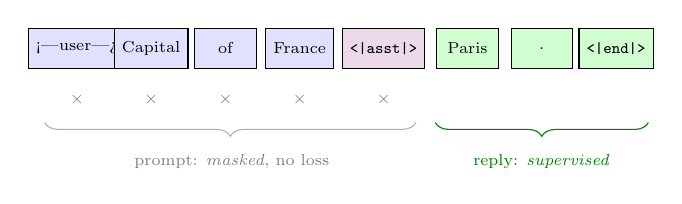
\begin{tikzpicture}[
      scale=0.82, every node/.style={scale=0.82},
      tok/.style={rectangle, draw, minimum width=0.95cm, minimum height=0.62cm, font=\scriptsize, align=center},
    ]
      % row of tokens: prompt (masked) then response (supervised)
      \node[tok, fill=blue!12] (a0) at (0, 0) {<|user|>};
      \node[tok, fill=blue!12] (a1) at (1.15, 0) {Capital};
      \node[tok, fill=blue!12] (a2) at (2.30, 0) {of};
      \node[tok, fill=blue!12] (a3) at (3.45, 0) {France};
      \node[tok, fill=violet!15] (a4) at (4.75, 0) {\ttfamily{\scriptsize<|asst|>}};
      \node[tok, fill=green!18] (a5) at (6.05, 0) {Paris};
      \node[tok, fill=green!18] (a6) at (7.20, 0) {.};
      \node[tok, fill=green!18] (a7) at (8.35, 0) {\ttfamily{\scriptsize<|end|>}};

      % masks below
      \foreach \x in {0,1.15,2.30,3.45,4.75} {
        \node[font=\scriptsize, text=gray] at (\x, -0.8) {$\times$};
      }
      \foreach \x in {6.05,7.20,8.35} {
        \node[font=\scriptsize, text=green!50!black] at (\x, -0.8) {\checkmark};
      }

      % braces
      \draw[decorate, decoration={brace, amplitude=5pt, mirror}, gray!60]
        (-0.5, -1.15) -- (5.25, -1.15);
      \node[font=\scriptsize, text=gray, align=center] at (2.4, -1.75)
        {prompt: \emph{masked}, no loss};
      \draw[decorate, decoration={brace, amplitude=5pt, mirror}, green!50!black]
        (5.55, -1.15) -- (8.85, -1.15);
      \node[font=\scriptsize, text=green!50!black, align=center] at (7.2, -1.75)
        {reply: \emph{supervised}};
    \end{tikzpicture}
  \end{center}

  \begin{itemize}[nosep]
    \item Prompt / user tokens are given as context but incur \emphdef{no gradient}: we do not
      want the model to learn to generate user questions.
    \item \emphdef{Loss}: $\displaystyle \mathcal{L} = -\!\!\sum_{t \in \text{assistant}} \!\!\log \pi_\theta(y_t \mid y_{<t})$
      \quad (mask $=0$ on prompt tokens).
  \end{itemize}
\end{frame}

% -----------------------------------------------------------------------
\begin{frame}{SFT in Practice}
  \begin{algorithm}[H]
  \small
  \caption{Supervised Fine-Tuning}
  \KwInput{Base model $\pi_\theta$, dialogue dataset $\mathcal{D}$, learning rate $\alpha$}
  \For{each conversation $(m_1, \ldots, m_n) \in \mathcal{D}$}{
    Format with chat template $\to$ token sequence $y_{1:T}$\;
    Build loss mask: $1$ on assistant tokens, $0$ elsewhere\;
    Forward pass, compute masked cross-entropy $\mathcal{L}$\;
    $\theta \leftarrow \theta - \alpha \, \nabla_\theta \mathcal{L}$\;
  }
  \end{algorithm}

  \vspace{0.3em}
  \begin{columns}[T]
    \begin{column}{0.5\textwidth}
      \textbf{Practical notes}
      \begin{itemize}[nosep]
        \item Small LR, few epochs (1--3): the model is already capable.
        \item Overfitting is easy $\Rightarrow$ watch held-out loss, keep data diverse.
        \item Full fine-tuning is costly; often done \emphdef{parameter-efficiently} (next slide).
      \end{itemize}
    \end{column}
    \begin{column}{0.5\textwidth}
      \textbf{What SFT does and does not do}
      \begin{itemize}[nosep]
        \item[\checkmark] Instruction following, response format, dialogue turns.
        \item[$\times$] Cannot teach \emph{what to avoid}: only shows good replies.
        \item[$\Rightarrow$] Preference alignment (RLHF / DPO) comes next.
      \end{itemize}
    \end{column}
  \end{columns}
\end{frame}

\subsection{Parameter-Efficient Fine-Tuning}

% -----------------------------------------------------------------------
\begin{frame}{Parameter-Efficient Fine-Tuning (PEFT): Motivation}
  \textbf{Fine-tuning is not only for chat.} SFT also specializes a base model to a domain:
  \begin{itemize}[nosep]
    \item Medicine, finance, code, law.
  \end{itemize}

  \vspace{0.3em}
  \textbf{But we are compute-constrained.} Full fine-tuning updates \emph{all} weights:
  \begin{itemize}[nosep]
    \item Gradients $+$ optimizer state for every parameter (Adam: $\sim\!3\times$ model in memory).
    \item A full model copy stored and served \emph{per task}.
  \end{itemize}

  \vspace{0.3em}
  \emphdef{PEFT idea}: freeze pretrained weights, train only a small add-on ($\ll 1\%$ of params).

  \vspace{0.2em}
  \textbf{What freezing the backbone buys us}
  \begin{itemize}[nosep]
    \item \emphdef{Limited hardware:} optimizer state only for the small module; fits a large model on one GPU.
    \item \emphdef{Many tasks / users:} one frozen backbone, swap a tiny per-task module at serve time.
    \item \emphdef{Fast iteration:} checkpoints of MBs not GBs; less overfitting on small data.
  \end{itemize}
\end{frame}

% -----------------------------------------------------------------------
\begin{frame}{PEFT: Low-Rank Adaptation (LoRA)}
  \begin{columns}[T]
    \begin{column}{0.42\textwidth}
      \begin{center}
        \begin{tikzpicture}[
          scale=0.82, every node/.style={scale=0.82},
          frozen/.style={rectangle, draw, rounded corners, fill=blue!12, minimum width=1.6cm, minimum height=0.9cm, align=center, font=\scriptsize},
          train/.style={rectangle, draw, rounded corners, fill=orange!25, minimum width=1.0cm, minimum height=0.6cm, align=center, font=\scriptsize},
          io/.style={font=\scriptsize},
          arr/.style={-{Stealth[length=4pt]}, thick},
        ]
          \node[io] (x) at (0, -1.7) {$x$};
          \node[frozen] (W) at (-1.3, 0) {$W$\\\tiny frozen};
          \node[train] (A) at (1.3, -0.9) {$A$};
          \node[train] (B) at (1.3, 0.4) {$B$};
          \node[circle, draw, inner sep=1pt, font=\scriptsize] (sum) at (0, 1.4) {$+$};
          \node[io] (h) at (0, 2.2) {$h$};
          \draw[arr] (x) -- (W.south);
          \draw[arr] (x) -| (A.south);
          \draw[arr] (A) -- (B);
          \draw[arr] (W.north) -- (sum);
          \draw[arr] (B.north) -- (sum);
          \draw[arr] (sum) -- (h);
          \node[font=\tiny, text=orange!70!black, align=center] at (2.7, -0.25) {rank $r$\\update $BA$};
        \end{tikzpicture}
      \end{center}
    \end{column}
    \begin{column}{0.56\textwidth}
      A weight update $\Delta W$ during fine-tuning has \emphdef{low intrinsic rank}. LoRA parametrizes it as a product of two thin matrices:
      \[
        h = Wx + \Delta W x = Wx + \frac{\alpha}{r}\,\underbrace{B A}_{\text{rank }\le r}\,x
      \]
      with $A \in \mathbb{R}^{r \times d}$, $B \in \mathbb{R}^{d \times r}$, $r \ll d$.
      \begin{itemize}[nosep]
        \item Freeze $W$, train only $A, B$: parameters drop from $d^2$ to $2rd$.
        \item $A$ random-init, $B = 0$ $\Rightarrow$ training starts exactly at the base model.
        \item Scaling $\tfrac{\alpha}{r}$: constant $\alpha$ decouples update size from $r$, so $r$ can be retuned without re-tuning the learning rate.
        \item Applied \emph{in parallel}, typically to attention projections $W_q, W_v$.
      \end{itemize}
    \end{column}
  \end{columns}

  \vspace{0.4em}
  \begin{itemize}[nosep]
    \item \emphdef{Merge at inference:} fold $W \leftarrow W + \tfrac{\alpha}{r}BA$ once training is done $\Rightarrow$ \emphdef{zero added latency}.
    \item \emphdef{Serve many tasks:} keep $W$ shared, load a different $(A,B)$ per task on the fly.
    \item Dominant PEFT method today; \emph{de facto} standard for community fine-tunes (LLMs and diffusion models).
  \end{itemize}
\end{frame}

% -----------------------------------------------------------------------
\begin{frame}{PEFT: Adapters}
  \begin{columns}[T]
    \begin{column}{0.4\textwidth}
      \begin{center}
        \begin{tikzpicture}[
          scale=0.82, every node/.style={scale=0.82},
          layer/.style={rectangle, draw, rounded corners, fill=blue!12, minimum width=2.0cm, minimum height=0.6cm, align=center, font=\scriptsize},
          train/.style={trapezium, draw, fill=orange!25, font=\scriptsize, align=center, trapezium stretches=true},
          arr/.style={-{Stealth[length=4pt]}, thick},
        ]
          \node[layer] (sub) at (0, 0) {Attn / FFN \tiny(frozen)};
          \node[train, trapezium angle=115, shape border rotate=180, minimum width=1.6cm] (down) at (0, 1.0) {down $d\to r$};
          \node[circle, draw, inner sep=0.5pt, font=\tiny] (nl) at (0, 1.75) {$\sigma$};
          \node[train, trapezium angle=115, minimum width=1.6cm] (up) at (0, 2.5) {up $r\to d$};
          \node[circle, draw, inner sep=1pt, font=\scriptsize] (sum) at (0, 3.4) {$+$};
          \draw[arr] (-1.8,-0.8) node[left, font=\scriptsize]{$x$} -| (sub.south);
          \draw[arr] (sub) -- (down);
          \draw[arr] (down) -- (nl);
          \draw[arr] (nl) -- (up);
          \draw[arr] (up) -- (sum);
          \draw[arr] (sum) -- ++(0,0.75) node[above, font=\scriptsize]{$h$};
          % residual taps off after the frozen sublayer
          \fill[gray] (0,0.5) circle (1.3pt);
          \draw[arr, gray] (0,0.5) -- (1.7,0.5) |- (sum.east);
          % adapter label on the left
          \draw[decorate, decoration={brace, amplitude=4pt, mirror}, orange!70!black]
            (-0.9, 2.85) -- (-0.9, 0.75)
            node[midway, left=2pt, font=\tiny, text=orange!70!black, align=center] {adapter\\(trained)};
        \end{tikzpicture}
      \end{center}
    \end{column}
    \begin{column}{0.58\textwidth}
      Insert a small \emphdef{bottleneck} module \emph{inside} each transformer block, after a sublayer:
      \[
        x \;\leftarrow\; x + W_{\text{up}}\,\sigma\!\left(W_{\text{down}}\, x\right)
      \]
      \begin{itemize}[nosep]
        \item Down-project $d \to r$, nonlinearity, up-project $r \to d$, then a residual connection.
        \item Only the adapter ($2rd$ params) is trained; the rest of the block is frozen.
        \item Near-zero init of $W_{\text{up}}$ $\Rightarrow$ starts as identity, does not disrupt the base model.
      \end{itemize}
    \end{column}
  \end{columns}

  \vspace{0.4em}
  \begin{description}[nosep]
    \item[vs.\ LoRA:] Adapters are \emphdef{sequential} (extra layers in the forward pass) so they add
      a little inference latency and \emph{cannot} be merged away. LoRA runs in parallel and merges to zero overhead.
  \end{description}
\end{frame}

% -----------------------------------------------------------------------
\begin{frame}{PEFT: Prefix and Prompt Tuning}
  Instead of modifying weights, \emphdef{prepend trainable vectors} to the input while the whole
  model stays frozen. The vectors steer the attention without touching any weight matrix.

  \vspace{0.3em}
  \begin{columns}[T]
    \begin{column}{0.42\textwidth}
      \begin{center}
        \begin{tikzpicture}[
          scale=0.8, every node/.style={scale=0.8},
          soft/.style={rectangle, draw, rounded corners, fill=orange!25, minimum width=0.55cm, minimum height=0.55cm, font=\scriptsize},
          tok/.style={rectangle, draw, rounded corners, fill=blue!12, minimum width=0.9cm, minimum height=0.55cm, font=\scriptsize},
          arr/.style={-{Stealth[length=4pt]}, thick},
        ]
          \node[soft] (p1) at (0, 0) {$p_1$};
          \node[soft] (p2) at (0.65, 0) {$p_2$};
          \node[soft] (p3) at (1.30, 0) {$p_3$};
          \node[tok] (t1) at (2.35, 0) {The};
          \node[tok] (t2) at (3.45, 0) {cat};
          \node[tok] (t3) at (4.45, 0) {\ldots};

          \draw[decorate, decoration={brace, amplitude=4pt}, orange!70!black]
            (-0.35, 0.45) -- (1.65, 0.45)
            node[midway, above=3pt, font=\tiny, text=orange!70!black] {trained};
          \draw[decorate, decoration={brace, amplitude=4pt}, blue!60]
            (1.85, 0.45) -- (4.95, 0.45)
            node[midway, above=3pt, font=\tiny, text=blue!60] {frozen tokens};

          \node[rectangle, draw, rounded corners, fill=blue!8, minimum width=5.3cm, font=\scriptsize] (model) at (2.3, -1.2) {Frozen Transformer};
          \foreach \n in {p1,p2,p3,t1,t2,t3} { \draw[arr, gray!60] (\n.south) -- (\n.south |- model.north); }
        \end{tikzpicture}
      \end{center}
    \end{column}
    \begin{column}{0.56\textwidth}
      \begin{description}[nosep]
        \item[Prompt tuning \cite{lester2021prompt}:] prepend $k$ learned embeddings (``soft prompt'') to the
          input only. Tiny ($k \cdot d$ params); works best at large scale.
        \item[Prefix tuning \cite{li2021prefix}:] prepend learned key/value vectors at \emph{every} layer.
          More capacity, more parameters.
      \end{description}
    \end{column}
  \end{columns}

  \vspace{0.4em}
  \begin{itemize}[nosep]
    \item No architecture change: the backbone is untouched, only the prepended vectors are trained.
    \item Costs \emphdef{context length}: soft tokens occupy positions in the sequence.
    \item Generally less expressive than LoRA / adapters; mostly of historical and conceptual interest.
  \end{itemize}
\end{frame}
